\section{Cơ chế hoạt động của hệ điều hành Android}

    Android được xây dựng dựa trên nhân Linux, tận dụng tính ổn định, bảo mật và khả năng quản lý tiến trình hiệu quả của hệ điều hành mã nguồn mở này. Mỗi ứng dụng Android hoạt động trong một tiến trình độc lập, có UID, máy ảo và vùng nhớ riêng, đảm bảo cách ly an toàn thông qua cơ chế sandbox. Android sử dụng máy ảo Dalvik (trước Android 5.0) và ART (từ Android 5.0 trở đi) để thực thi mã ứng dụng, giúp tăng hiệu suất và bảo mật. Nhờ kiến trúc này, Android có thể bảo vệ người dùng khỏi các ứng dụng độc hại và tối ưu hóa tài nguyên hệ thống.
% 2.1
\subsection{Android trên nền tảng Linux}
\renewcommand{\labelitemi}{--}    
    Android được xây dựng trên nhân (kernel) của hệ điều hành Linux, tức là sử dụng Linux kernel làm lớp điều khiển phần cứng như quản lý bộ nhớ, tiến trình, thiết bị ngoại vi và bảo mật hệ thống. Trong khi đó, các thành phần còn lại như giao diện người dùng, framework ứng dụng và dịch vụ hệ thống đều do Google phát triển riêng biệt, không sử dụng giao diện truyền thống của Linux. Android chọn Linux kernel vì đây là nền tảng mã nguồn mở, ổn định, có tính bảo mật cao và hỗ trợ tốt cho các tính năng quan trọng của thiết bị di động như xử lý đa tiến trình, cấp quyền truy cập theo người dùng và hỗ trợ phần cứng đa dạng. Việc kế thừa nhân Linux giúp Android tăng tính linh hoạt, tiết kiệm thời gian phát triển và dễ dàng tùy biến cho từng nhà sản xuất thiết bị.\\
    \begin{figure}[H] 
            \centering
            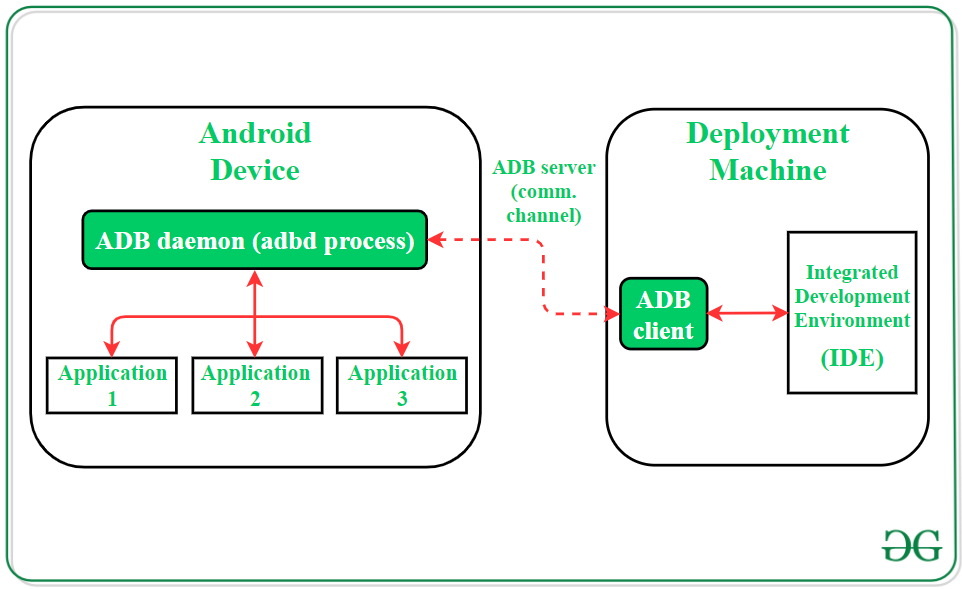
\includegraphics[width=0.7\textwidth]{images/app-work.png}
            \caption{Thiết lập máy chủ ADB~\cite{app-working}.}
            \label{fig:android4}
        \end{figure}
    Google đã tùy biến kernel Linux để phù hợp hơn với điện thoại:
    \begin{table}[H]
        \centering
        \renewcommand{\arraystretch}{1.5}
        \begin{tabular}{|p{3.5cm}|p{10cm}|}
            \hline
            \textbf{Tính năng bổ sung} & \textbf{Công dụng} \\
            \hline
            WakeLocks & Cho phép ứng dụng hoặc hệ thống giữ CPU không rơi vào trạng thái ngủ khi cần thực hiện các tác vụ nền quan trọng, giúp tiết kiệm pin một cách chủ động. \\
            \hline
            Ashmem  & Cung cấp cơ chế chia sẻ vùng nhớ tạm thời giữa các tiến trình, cho phép truyền dữ liệu hiệu quả mà không cần lưu vào bộ nhớ lâu dài. \\
            \hline
            Binder IPC & Là hệ thống giao tiếp liên tiến trình (Inter-Process Communication) do Android phát triển, dùng để truyền dữ liệu và lệnh giữa các app và dịch vụ hệ thống một cách an toàn và nhanh chóng. \\
            \hline
            Logger & Ghi lại thông tin log hệ thống, giúp nhà phát triển theo dõi, phân tích lỗi và hoạt động của ứng dụng hoặc hệ điều hành. \\
            \hline
            Alarm Drivers & Quản lý các sự kiện báo thức (alarm) trong hệ thống, cho phép ứng dụng thực thi tác vụ định kỳ hoặc vào một thời điểm nhất định, kể cả khi thiết bị đang ở trạng thái nghỉ. \\
            \hline
        \end{tabular}
        \caption{Các tính năng Google thêm vào Linux để hỗ trợ hệ điều hành Android~\cite{kernel-linux}.}
        \label{table:android-linux-features}
        \end{table}          

\renewcommand{\labelitemi}{--}    
        Mỗi ứng dụng gắn với một định danh người dùng riêng. UID (User ID) là mã định danh người dùng cấp hệ điều hành. Trong Android, mỗi ứng dụng (app) được xem như một người dùng độc lập, và hệ thống cấp cho nó một UID riêng biệt.
        \setlength{\leftmargini}{1.5cm}
        \begin{itemize}
            \item Nguồn gốc của UID trong Android bắt nguồn từ nền tảng hệ điều hành Linux, vì Android được xây dựng trên nhân Linux. Linux vốn là một hệ điều hành hỗ trợ mô hình đa người dùng, trong đó mỗi người dùng được xác định duy nhất bởi một UID – một số nguyên đặc trưng cho từng user. Trong môi trường Linux, mọi tiến trình đều chạy dưới quyền của một người dùng cụ thể, và hệ thống sử dụng UID để xác định quyền truy cập của tiến trình đó tới các tài nguyên như tệp tin, thiết bị, vùng nhớ và các tiến trình khác. Android đã kế thừa và phát triển mô hình này để áp dụng vào môi trường di động: thay vì một người dùng thực sự, mỗi ứng dụng Android được coi như một "người dùng" riêng biệt, và được gán một UID duy nhất bởi hệ thống tại thời điểm cài đặt. Việc cấp UID riêng cho mỗi ứng dụng không chỉ giúp cách ly dữ liệu giữa các ứng dụng mà còn ngăn chặn hành vi truy cập trái phép vào bộ nhớ hoặc tài nguyên hệ thống. Cơ chế này là nền tảng quan trọng cho mô hình sandbox trong Android, tạo ra một môi trường chạy độc lập và an toàn cho mỗi ứng dụng, đồng thời tận dụng tối đa các cơ chế kiểm soát truy cập đã được Linux xây dựng sẵn.
            \item Mỗi ứng dụng đều có vùng dữ liệu riêng nằm trong thư mục /data/data/<tên gói> và chỉ tiến trình chạy dưới UID tương ứng với ứng dụng đó mới có quyền truy cập. Các ứng dụng khác không thể truy cập trực tiếp vào dữ liệu này, trừ khi được cấp phép thông qua hệ thống quyền (permissions) và các cơ chế kiểm soát quyền truy cập như tập tin, cơ sở dữ liệu hoặc socket.
        \end{itemize}

        \begin{figure}[H] 
            \centering
            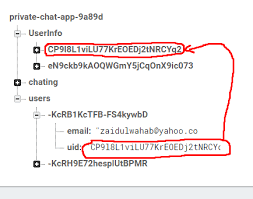
\includegraphics[width=0.5\textwidth]{images/uid.png}
            \caption{So sánh UID với khóa con khác~\cite{compare-uid}.}
            \label{fig:android5}
        \end{figure}

% 2.2
\subsection{Cơ chế sandbox}
\renewcommand{\labelitemi}{--}    
        Sandbox trong Android là một môi trường cách ly, nơi mỗi ứng dụng (app) được “nhốt” vào một không gian riêng biệt, không thể trực tiếp can thiệp hay truy cập vào dữ liệu hoặc tiến trình của ứng dụng khác. Hình dung như mỗi app sống trong một “phòng riêng” với cửa khóa, không ai ra vào nếu không có chìa khóa (quyền được cấp) \cite{app-sandbox}. Cách Android thực hiện sandbox là kết hợp nhiều công nghệ.
        \setlength{\leftmargini}{1.5cm}
        \begin{table}[H]
            \centering
            \renewcommand{\arraystretch}{1.5}
            \begin{tabular}{|p{4.5cm}|p{9cm}|}
                \hline
                \textbf{Cơ chế bảo mật} & \textbf{Mục đích} \\
                \hline
                UID riêng biệt & Mỗi ứng dụng được gán một mã định danh người dùng (UID) riêng biệt, giúp chạy như một "user" độc lập trên nền tảng Linux, cách ly tài nguyên giữa các ứng dụng. \\
                \hline
                Filesystem permissions & Quyền truy cập hệ thống tệp tin được kiểm soát để mỗi ứng dụng chỉ có thể truy cập vào vùng dữ liệu riêng của nó, chẳng hạn như thư mục `/data/data/com.example.app`. \\
                \hline
                Máy ảo (VM) & Mỗi ứng dụng chạy trong một máy ảo riêng (trước đây là Dalvik, hiện tại là ART), giúp cách ly mã thực thi và tăng tính an toàn khi xử lý mã bytecode. \\
                \hline
                Permission system & Nếu ứng dụng muốn truy cập các tài nguyên hệ thống ngoài vùng sandbox như camera, GPS, microphone, hệ thống sẽ yêu cầu xin quyền rõ ràng từ người dùng. \\
                \hline
                SEAndroid & Dựa trên SELinux, SEAndroid (Security-Enhanced Android) bổ sung chính sách bảo mật ở cấp nhân hệ điều hành, kiểm soát hành vi truy cập tài nguyên của từng ứng dụng theo nguyên tắc quyền tối thiểu \cite{Android-Security-Overview}. \\
                \hline
            \end{tabular}
            \caption{Các cơ chế trong Android đảm bảo môi trường sandbox cho mỗi ứng dụng~\cite{app-sandbox}.}
            \label{table:android-sandbox-mechanisms}
            \end{table}
            
\newpage
    Sandbox bảo vệ những thứ sau:
      \setlength{\leftmargini}{1.5cm}
      \begin{itemize}
          \item Dữ liệu app (database, file, cache...): Không app nào khác có thể truy cập nếu không được cấp quyền
            \item Mã nguồn (classes.dex): Không bị sửa đổi/thay thế bởi app khác
            \item Giao tiếp giữa app: Chỉ có thể qua các cơ chế an toàn như Intent, ContentProvider, Binder
            \item Tài nguyên hệ thống (camera, GPS, v.v.): Chỉ truy cập được nếu người dùng cho phép thông qua hệ thống permission
        \end{itemize}
        
        \vspace{0.5em}
        Ví dụ: Giả sử có 2 app:
        App1 là ghi chú cá nhân,
        App2 là trò chơi.
        Cơ chế bảo vệ làm cho App2 không thể đọc được ghi chú của App1, trừ khi App1 cung cấp dữ liệu qua Intent, ContentProvider.

        \vspace{0.5em}

        Tóm lại, Sandbox là lá chắn vô hình bảo vệ mỗi ứng dụng Android như một thế giới riêng biệt. Nó giúp người dùng yên tâm cài đặt nhiều ứng dụng mà không sợ bị can thiệp trái phép.

% 2.3
\subsection{Máy ảo (VM) riêng cho mỗi ứng dụng}

  Máy ảo là một chương trình mô phỏng một hệ thống máy tính khác, cho phép chạy phần mềm như thể đang chạy trực tiếp trên một máy vật lý. Máy ảo không tương tác trực tiếp với phần cứng, mà thay vào đó hoạt động như một lớp trung gian giữa phần mềm và phần cứng thật. Mỗi máy ảo có môi trường thực thi riêng biệt, được cách ly hoàn toàn, giúp đảm bảo an toàn, ổn định và khả năng quản lý tài nguyên hiệu quả. Trong Android, máy ảo (cụ thể là Dalvik VM hoặc Android Runtime – ART) giữ vai trò trung gian để chạy các ứng dụng Android được biên dịch dưới dạng bytecode. Mã bytecode này được đóng gói trong tệp .dex, và là thành phần quan trọng nằm trong gói cài đặt ứng dụng .apk. Nhờ máy ảo, các ứng dụng có thể được chạy một cách độc lập, không ảnh hưởng đến các ứng dụng khác và bị giới hạn trong vùng tài nguyên mà hệ điều hành cho phép, giúp thực hiện cơ chế sandbox hiệu quả. Máy ảo cũng là yếu tố giúp hệ thống có khả năng phát hiện, cô lập lỗi và ngăn chặn hành vi xâm nhập không mong muốn từ ứng dụng độc hại.

  \vspace{0.5em}

  Dalvik VM ($Android \leq 4.x$): Là máy ảo đầu tiên của Android,  được thiết kế để chạy các ứng dụng Android trên các thiết bị di động với tài nguyên hạn chế. Dalvik sử dụng register-based architecture, khác với các máy ảo khác như Java Virtual Machine (JVM) vốn dựa trên stack-based architecture. Điều này có nghĩa là phần lớn các phép toán trong Dalvik được thực hiện trên các thanh ghi thay vì bộ nhớ, giúp giảm độ phức tạp và tối ưu hóa hiệu suất. Dalvik còn sử dụng Just-In-Time (JIT) compilation, nghĩa là mã ứng dụng được biên dịch thành mã máy khi ứng dụng đang chạy, thay vì biên dịch toàn bộ trước khi cài đặt. Điều này giúp tiết kiệm bộ nhớ và rút ngắn thời gian cài đặt ứng dụng, vì không cần biên dịch mã trước khi triển khai. Tuy nhiên, Dalvik cũng có một số nhược điểm. Quá trình khởi động ứng dụng có thể bị chậm vì mã phải được biên dịch khi chạy, dẫn đến trải nghiệm người dùng không mượt mà. Bên cạnh đó, hiệu suất tổng thể của Dalvik cũng không cao bằng các máy ảo khác, vì việc biên dịch mã trong thời gian chạy có thể gây ra sự chậm trễ trong quá trình thực thi ứng dụng. Mặc dù vậy, Dalvik vẫn là nền tảng quan trọng trong sự phát triển của Android cho đến khi được thay thế bởi ART (Android Runtime) trong các phiên bản Android sau này.
  Dùng từ Android 1.0 đến Android 4.4 (KitKat) \cite{art-dalvik}.
  \begin{figure}[H] 
    \centering
    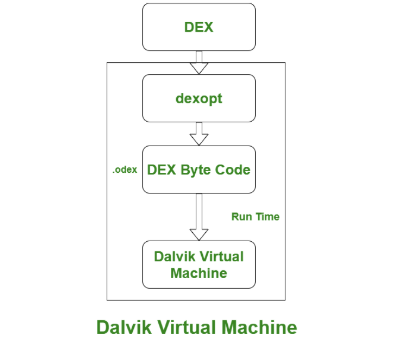
\includegraphics[width=0.6\textwidth]{images/DalvikVM.png}
    \caption{Máy ảo Dalvik~\cite{dalvik-and-art}.}
    \label{fig:android6}
\end{figure}  

    ART (Android Runtime): Thay thế Dalvik từ Android 5.0 (Lollipop), dùng AOT (Ahead-Of-Time) compilation để mã được biên dịch thành mã máy ngay khi cài app.
    Lợi ích là khởi chạy nhanh, hiệu suất cao.
    Nhược điểm là cài đặt lâu hơn, chiếm nhiều bộ nhớ.
    Sau Android 7.0, ART còn hỗ trợ thêm JIT lẫn AOT do đó tối ưu thời gian chạy lẫn bộ nhớ \cite{art-dalvik}.   
    \begin{figure}[H] 
        \centering
        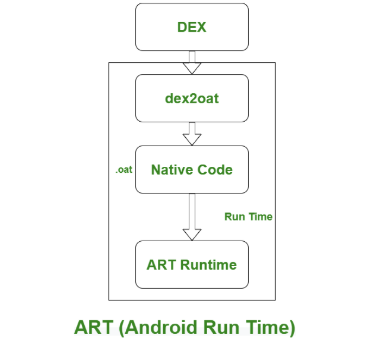
\includegraphics[width=0.6\textwidth]{images/ART.png}
        \caption{Android Run Time~\cite{dalvik-and-art}.}
        \label{fig:android}
    \end{figure}  
\newpage
    Quy trình thực thi của Dalvik VM và ART:
    \begin{table}[H]
        \centering
        \renewcommand{\arraystretch}{1.5}
        \begin{tabular}{|p{4cm}|p{5cm}|p{5cm}|}
        \hline
        \textbf{Giai đoạn} & \textbf{Dalvik VM} & \textbf{ART (Android Runtime)} \\
        \hline
        Khi cài đặt ứng dụng & Chép file \texttt{.dex} vào hệ thống & Biên dịch \texttt{.dex} thành mã máy \texttt{.oat} \\
        \hline
        Khi chạy ứng dụng & Dịch bytecode thành mã máy trong thời gian thực (JIT) & Chạy mã máy đã được biên dịch sẵn (AOT) \\
        \hline
        Khi mở lại ứng dụng & Vẫn phải dịch lại bytecode & Khởi động rất nhanh, không cần biên dịch lại \\
        \hline
        \end{tabular}
        \caption{So sánh quá trình thực thi ứng dụng giữa Dalvik VM và ART~\cite{dalvik-and-art}.}
        \label{tab:dalvik-vs-art}
        \end{table}
          
    Lý do Google chuyển từ Dalvik sang ART: Hiệu suất tăng mạnh (app khởi động nhanh hơn), tiết kiệm pin hơn, tối ưu RAM và bộ nhớ tốt hơn, chuẩn bị cho tương lai với các công nghệ như: Android Instant Apps, Dynamic Delivery.

\renewcommand{\labelitemi}{--} 
        \vspace{0.5em}  
        Mỗi ứng dụng là một tiến trình độc lập. Trong Android, mỗi ứng dụng (app) khi được khởi chạy sẽ được cấp phát một tiến trình riêng biệt (process). Tiến trình này có vùng nhớ riêng, UID riêng, máy ảo riêng, hoạt động độc lập, không can thiệp lẫn nhau.
      \setlength{\leftmargini}{1.5cm}
      \begin{itemize}
        \item Lợi ích: App không thể truy cập dữ liệu, bộ nhớ hay tiến trình của app khác (bảo mật), nếu 1 app lag/crash, không ảnh hưởng app khác (tối ưu hiệu năng), có thể theo dõi, dừng, hoặc khởi động lại tiến trình một cách riêng lẻ (quản lí tài nguyên), khi hệ thống cần RAM, Android có thể tắt tiến trình app ít dùng mà không ảnh hưởng toàn hệ thống (tự động giải phóng)
        \item Android tạo ra một tiến trình mới: khi người dùng mở ứng dụng lần đầu, app được khởi động lại sau khi bị hệ thống giải phóng
        \item Vùng nhớ riêng trong mỗi tiến trình: mỗi tiến trình chỉ "thấy" được biến, đối tượng trong phạm vi của nó, dữ liệu trong thư mục app, không thể trực tiếp truy cập đến vùng nhớ của tiến trình khác (do cơ chế sandbox, UID, VM kết hợp bảo vệ).
      \end{itemize}
